\begin{frame}{}
    \LARGE Advanced Diffusion Models: \textbf{PDE-based Diffusion Models}
\end{frame}

\begin{frame}[allowframebreaks]{PDE-based Diffusion Models}
    \begin{itemize}
        \item Leverage diffusion models, originally for image generation, to solve and analyze PDEs.
        \item Learn complex PDE relationships by adding noise to solutions and reversing the process.
        \item Effective for handling incomplete or uncertain data.
        \item Valuable in scientific and engineering applications.
    \end{itemize}

    \framebreak
    % \textbf{Key Concepts}
    % \begin{itemize}
    %     \item \textbf{PDEs:} Partial Differential Equations, fundamental in modeling physical phenomena.
    %     \item \textbf{Diffusion Process:} Gradually adds noise to PDE solutions, then learns to reverse this process.
    %     \item \textbf{Data Handling:} Can work with incomplete or noisy data, making it robust for real-world applications.
    % \end{itemize}

    \textbf{Core Idea}
    \begin{itemize}
        \item Diffusion models transform data into a simple distribution (e.g., Gaussian noise) via a forward process.
        \item A reverse process is learned to reconstruct the original data from noise.
        \item For PDEs, the model maps input or boundary conditions to PDE solutions, capturing the equation's dynamics.
    \end{itemize}
\end{frame}

\begin{frame}{Why Use Diffusion Models for PDEs?}
    \begin{itemize}
        \item \textbf{Generative Solutions:} Can produce multiple plausible PDE solutions, useful under uncertainty or incomplete information.
        \item \textbf{Uncertainty Modeling:} Capture a distribution of possible solutions, not just a single answer.
        \item \textbf{Partial Data Learning:} Train effectively on datasets with missing or incomplete data, suitable for real-world scenarios.
        \item \textbf{Flexibility:} Adaptable to both forward (solving PDEs) and inverse (parameter estimation) problems.
    \end{itemize}
\end{frame}

\begin{frame}[allowframebreaks]{DiffusionPDE}
    % \frametitle{Diffusion Partial Differential Equation (PDE)}

    The diffusion equation is a fundamental PDE describing the distribution of a quantity (such as heat or particles) diffusing through a medium:
    \begin{equation}
        \frac{\partial u}{\partial t} = D \nabla^2 u
    \end{equation}
    where:
    \begin{itemize}
        \item $u = u(\mathbf{x}, t)$ is the quantity of interest (e.g., concentration, temperature)
        \item $D$ is the diffusion coefficient
        \item $\nabla^2$ is the Laplacian operator
    \end{itemize}

    \framebreak

    \begin{figure}
        \centering
        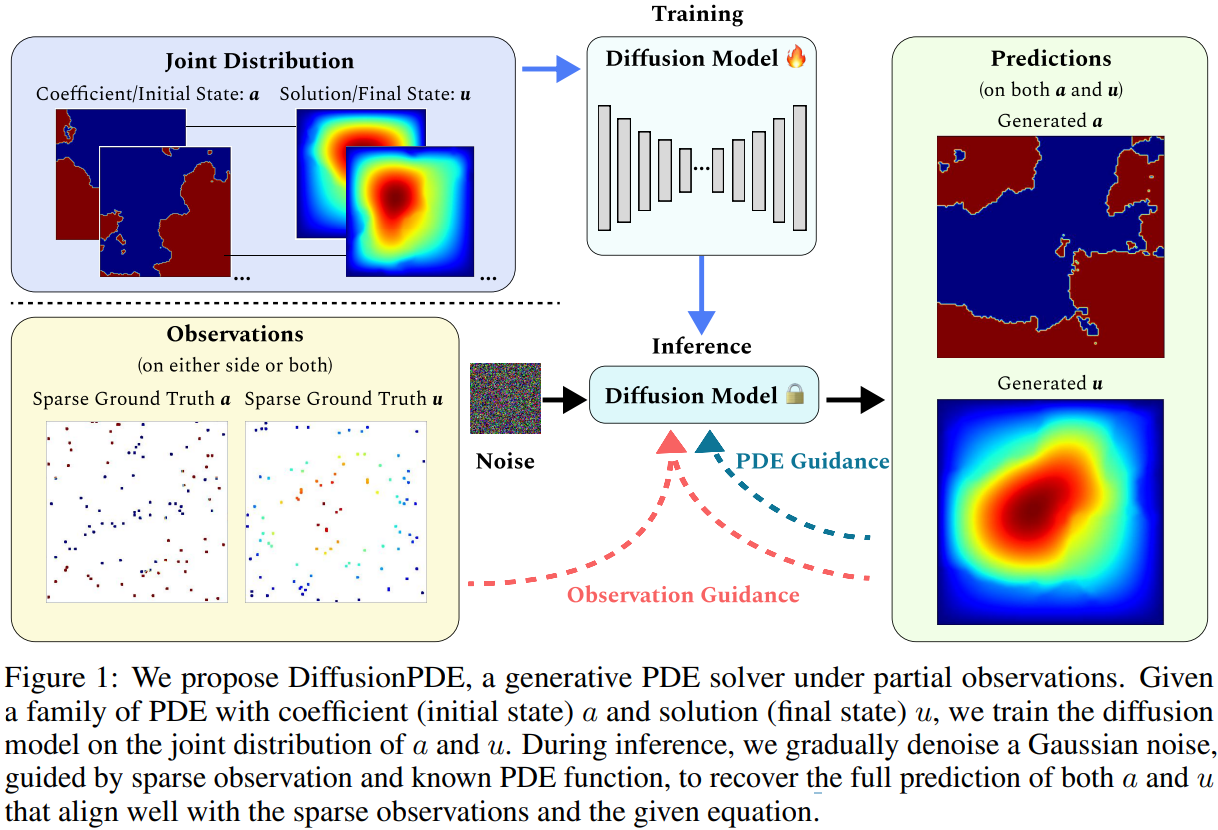
\includegraphics[width=\linewidth,height=\textheight,keepaspectratio]{images/adv-img-gen/diffusionpde-1.png}
    \end{figure}

    \framebreak

    \begin{figure}
        \centering
        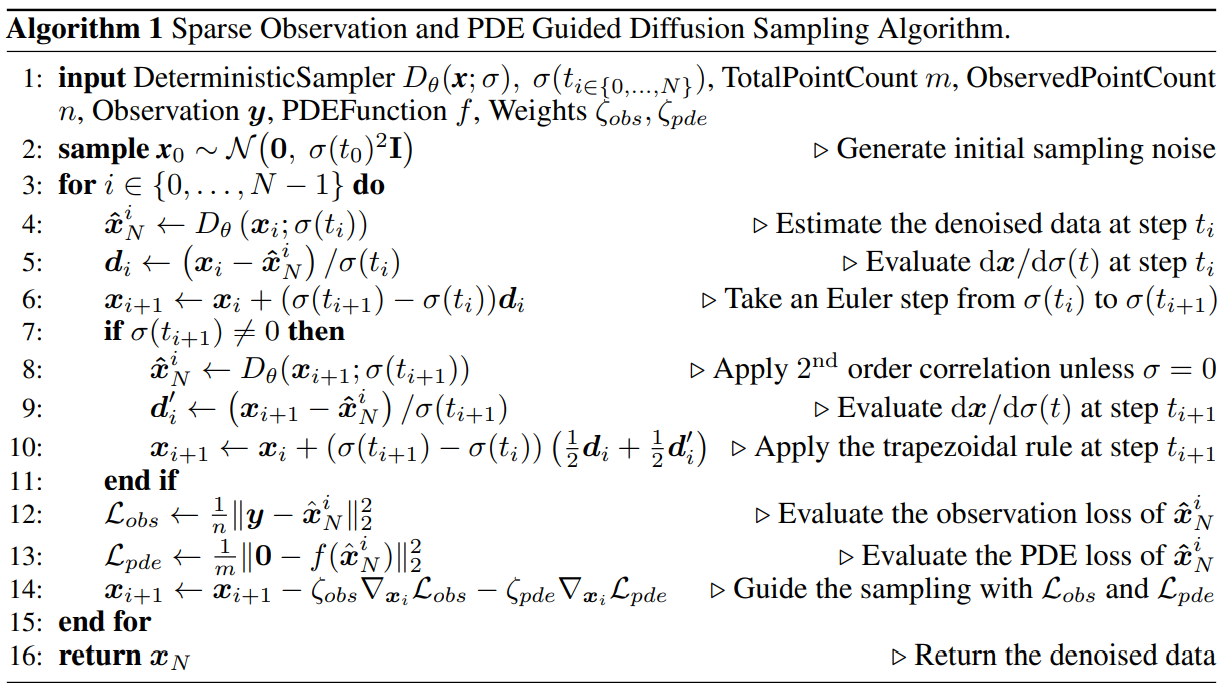
\includegraphics[width=\linewidth,height=\textheight,keepaspectratio]{images/adv-img-gen/diffusionpde-algo-1.png}
    \end{figure}

    \framebreak

    \begin{figure}
        \centering
        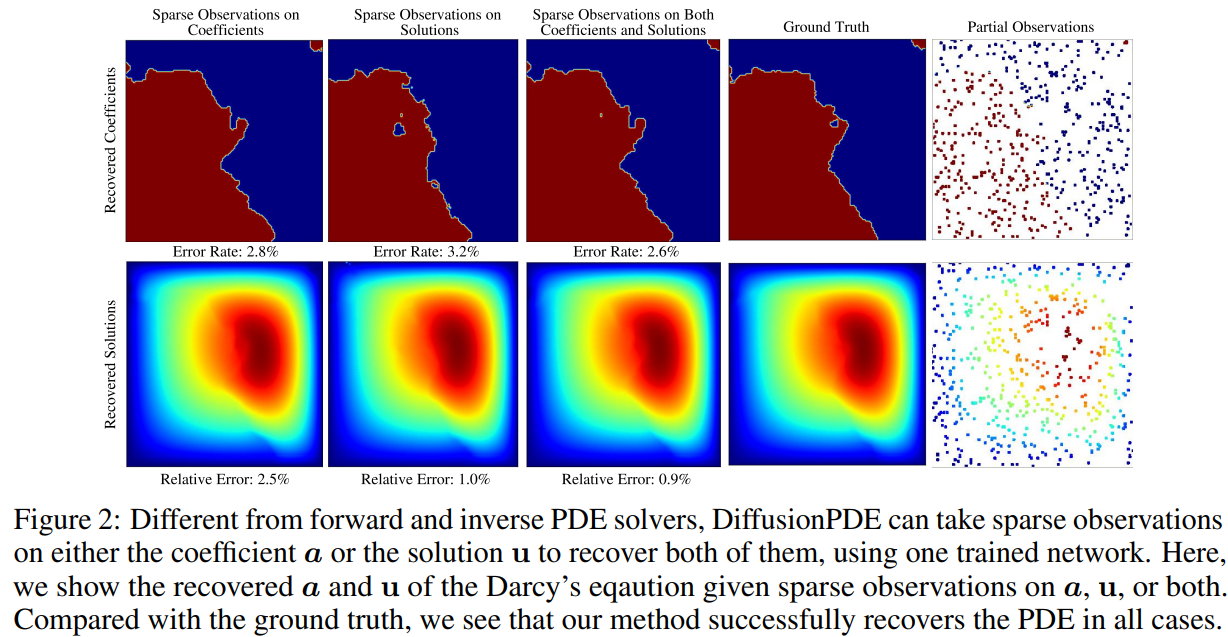
\includegraphics[width=\linewidth,height=\textheight,keepaspectratio]{images/adv-img-gen/diffusionpde-2.png}
    \end{figure}

    \framebreak

    \begin{figure}
        \centering
        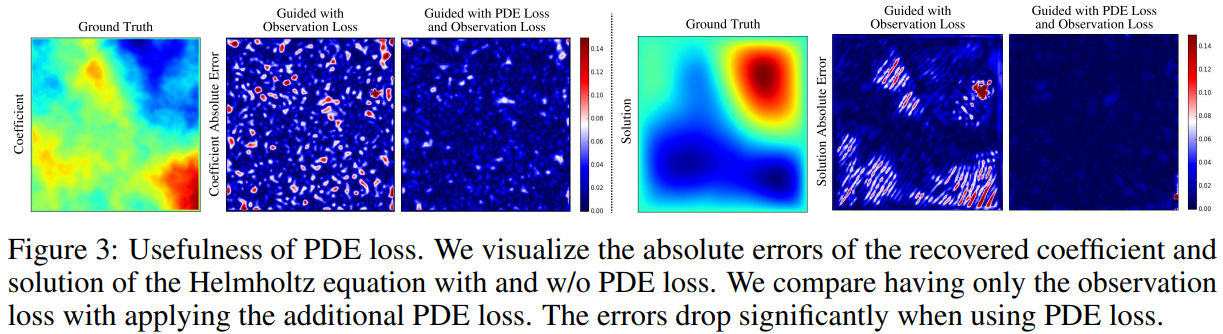
\includegraphics[width=\linewidth,height=\textheight,keepaspectratio]{images/adv-img-gen/diffusionpde-3.png}
    \end{figure}
\end{frame}

